\documentclass[11pt,a5paper]{article}

\usepackage[T1]{fontenc}
\usepackage[utf8]{inputenc}
\usepackage{lmodern, microtype}
\usepackage[estonian]{babel}
\usepackage[per=fraction, expproduct=cdot, decimalsymbol=comma, inter-unit-product=\cdot]{siunitx}
\usepackage{graphicx}
\usepackage{wrapfig}
\usepackage{subfig}
\usepackage{tikz}
\usepackage[european]{circuitikz}
\tikzset{component/.style={draw,thick,circle,fill=white,minimum size=0.75cm,inner sep=0pt}}
\usepackage{amsmath,amssymb}
\usepackage{amsfonts}
\usepackage{hyperref}
\usepackage{csquotes}
\usepackage{caption}
\usepackage{enumitem}
\topmargin=-3.0cm \textheight=19cm \textwidth=12.9cm
\oddsidemargin=-1.5cm  \evensidemargin=-1.5cm
\setlength{\parindent}{0pt} \setlength{\parskip}{6pt} \sloppy
\sloppy \relpenalty=10000 \binoppenalty=10000
\pagestyle{empty}

\newcommand{\numb}[1]{\vspace{5pt}\textbf{\large #1}}
\newcommand{\nimi}[1]{(\textsl{\small #1})}
\newcommand{\punktid}[1]{(\emph{#1~p.})}
\newcounter{ylesanne}
\newcommand{\yl}[1]{\addtocounter{ylesanne}{1}\numb{\theylesanne.} \nimi{#1} \newblock{}}
\newcommand{\autor}[1]{}
% \newcommand{\autor}[1]{\emph{ Autor: #1}} %Temporarily surpressed

\begin{document}
\begin{center}
  \textbf{\Large Eesti koolinoorte 68. füüsikaolümpiaad} \par
  \emph{10. aprill 2021. a. Lõppvoor \\Gümnaasiumi ülesanded (10.--12. klass)}
\end{center}

\resizebox{\textwidth}{!}{
  \emph{%
    \begin{tabular}{@{}l@{}}
      \textbf{Palun kirjutada iga ülesande lahendus eraldi lehele ning skaneerida eraldi failidesse.}\\
      Lahendamisaeg on 5 tundi. \\
      Iga osavõtja võib lahendada kõiki pakutud ülesandeid. \\
      Arvesse lähevad 5 suurima punktide arvu saanud teoreetilist ja 1 eksperimentaalne ülesanne. \\
      Kasutada võib kirjutus- ja joonestusvahendeid ning kalkulaatorit. Muud abivahendid on keelatud.\\
      Eksperimentaalülesande lahendamisel võib kasutada üksnes loetelus toodud vahendeid. \\
      Mõõtemääramatuse hindamist ei nõuta.
    \end{tabular}
  }
} \par

\yl{LUMEPALL}
Hannes istub $H=\SI{7.7}{\m}$ kõrgusel puu otsas ja tal on käes lumepall. Ta märkab otse tema suunas kiirusega $v=\SI{6.0}{\km\per\hour}$ lähenevat Richardit, kes on puust $l=\SI{7.0}{\m}$ kaugusel, ja otsustab teda lumepalliga visata. Millise kiirusega peaks ta lumepalli horisontaalselt viskama, et tabada Richardi pead, kui Richard on $h=\SI{1.8}{\m}$ pikk? Raskuskiirendus $g=\SI{9.8}{\m\per\s\squared}$.
\punktid{6} \autor{Oleg Košik}

\yl{PUDEL}
Pärast kuumal päeval õues treenimist tuli sportlane oma tühja õrnast plastmassist joogipudeliga jahedasse tuppa ning ta märkas, et ta pudel hakkas vaikselt \enquote{paukuma}. Lähemal uurimisel selgus, et kui pudeli sisene rõhk erineb välisest rõhust suuruse $\Delta p$ võrra, siis tekib pudeli kesta sisse üks lohukujuline mõlk juurde (selle tekkimine kostuski pauguna) ning hetkeks võrdsustuvad sise- ja välisrõhud. Sportlane mõõtis kahe paugu vaheliseks ajaks $t$. Leidke pudeli soojuskadude võimus vahetult pärast pudeli tuppa toomist. Tühja pudeli (seal hulgas pudelis oleva õhu) soojusmahutavus on $c$, õhu molaarruumala on $V_m$ ja universaalne gaasikonstant on $R$. Võib eeldada, et ajavahemiku $t$ jooksul soojuskadude võimus ei muutu.
\punktid{6} \autor{Jarl Patrick Paide}

\yl{LÄÄTS JA EKRAAN}
Jarl asetas punktvalgusallika ja ekraani vahele õhukese kumerläätse (raamita klaaslääts); valgusallikas asus peateljel ja ekraani tasand oli paralleelne läätse tasandiga. Ta liigutas ekraani edasi-tagasi, uurides sellel tekkivat mustrit ning pani tähele, et kui ekraan asub läätsest kaugusel \SI{10}{\cm}, tekib ekraanile terav valgusallika kujutis. Üllatuslikult selgus, et kui ekraani kaugus läätsest oli \SI{60}{\cm}, siis ei olnud seal näha enam mingit mustrit: ekraan oli ühtlase heledusega nagu läätse polnukski!\\
\osa Leidke läätse fookuskaugus.\\
\osa Mis kujuga muster tekib ekraanile, kui ekraan asub kaugemal, kui \SI{10}{\cm} läätsest, kuid lähemal, kui \SI{60}{\cm} läätsest?
\punktid{8} \autor{Oleg Košik}

\newpage
\yl{SÕIT JÄÄL} Kaarel sõidab autoga libedal horisontaalsel teel pikkusega $2L=\SI{100}{\m}$. Tee koosneb kahest lõigust: esimesel lõigul pikkusega $L=\SI{50}{\m}$ on rataste ja maapinna vaheline hõõrdetegur $\mu_1=\SI{0.1}{}$ ja teisel lõigul pikkusega $L=\SI{50}{\m}$ on hõõrdetegur $\mu_2=\SI{0.2}{}$. Alguses on Kaarli auto esimese lõigu alguses paigal. Ta tahab tee läbida võimalikult kiiresti, nii et auto jääks täpselt teise lõigu lõpus seisma. Leidke minimaalne võimalik tee läbimise aeg. Raskuskiirenduse väärtuseks võtta $g=\SI{10}{\m\per\s\squared}$.
\punktid{8} \autor{Richar Luhtaru}

\yl{VÕIMSUS}
Juuresoleval skeemil on alguses lüliti avatud. Leidke takistitel eralduv koguvõimsus \\
\osa vahetult pärast lüliti sulgemist; \\
\osa pika aja möödudes pärast lüliti sulgemist.\\
Kõikide takistite takistus on $R$ ja patarei pinge on $V$.
\punktid{8} \autor{Kaur Aare Saar}
\vspace{-4pt}
\begin{figure}[h]
  \centering
  \begin{minipage}[h]{0.44\textwidth}
    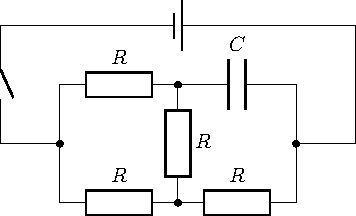
\includegraphics[width=\textwidth]{skeem.pdf}
  \end{minipage}
 \end{figure}
\vspace{-12pt}

\yl{KEHA KERAL}
Kerakujulisele, ühtlase massijaotusega planeedile, raadiusega $R$, massiga $M$ ja pöörlemisperioodiga $T$ asetatakse väikese massiga keha $m$. Gravitatsioonikonstant on G.\\
\osa Leia väikese keha kaal funktsioonina laiuskraadist $\theta$.\\
\osa Leia hõõrdeteguri $\mu$ väärtuste vahemik funktsioonina laiuskraadist $\theta$, mille puhul püsib väike keha planeedi peal staatilisena. \par
\emph{Märkus:} laiuskraadi $\theta$ mõõdetakse ekvaatorilt.
\punktid{10} \autor{Krister Kasemaa}

\yl{KOLMNURK}
Kolm ühesuguse massiga $m$ osakest paigutatakse punktidesse $A$, $B$ ning $C$. Osakeste mõõtmed on palju väiksemad kolmnurga $ABC$ küljepikkustest $a=|BC|$, $b=|CA|$ ja $c=|AB|$. Osake punktis $A$ kannab laengut $q_A$, osake punktis $B$ --- laengut $q_B$ ja osake punktis $C$ --- laengut $q_C$. Osakesed vabastatakse ning need hakkavad paigalseisust liikuma elektrostaatilise vastasmõju tõttu.\\
\osa Millised peaksid olema laengute suhted, et kõigi osakeste trajektoorid oleksid sirgjooned?\\
\osa Kas sirgjooneline liikumine on võimalik suvalise kolmnurga $ABC$ puhul?
\punktid{10} \autor{Jaan Kalda}

\yl{VEESILINDER}
Mihkel täidab silindrilise anuma kõrgusega $h = \SI{12}{\m}$ täielikult veega. Seejärel ta katab silindri kaanega, ning pöörab selle tagurpidi. Missuguse kiirendusega hakkab vesi silindrist välja voolama, kui Mihkel silindri alt kaane ära võtab? Küllastunud veeauru rõhk toatemperatuuril on $p_v = \SI{3170}{\Pa}$, vee tihedus $\rho = \SI{1000}{\kg\per\m\cubed}$, atmosfääri rõhk $p_0 = \SI{101325}{\Pa}$, raskuskiirendus $g = \SI{9.8}{\m\per\s\squared}$.
\punktid{12} \autor{Taavet Kalda}

\yl{VEDELIK PEEGLIL}
Laua peal lebab veega täidetud sfääriline nõguspeegel, kusjuures vesi ulatub peegli servani (vt joonist). Peegli kohale kõrgusele $h=\SI{25.0}{cm}$ on kinnitatud valgusallikas nii, et selle kujutis kattub allikaga. Seejärel asendatakse vesi tundmatu vedelikuga, mille peale nihkub kujutis $l=\SI{5.0}{cm}$ võrra peegli poole. Leidke tundmatu vedeliku murdumisnäitaja. Eeldada, et peegli laius on palju väiksem kui $l$, $h$, s.t. võib kasutada väikeste nurkade lähendust $\sin \alpha \approx \tan \alpha \approx \alpha$, kus $\alpha$ on radiaanides. Vee murdumisnäitaja on $n_v=\num{1.33}$.
\punktid{12} \autor{Konstantis Dukatš}
\begin{figure}[h]
  \centering
  \begin{tikzpicture}
    \fill [fill opacity=0.2, fill=blue] (0,0) arc (240:300:6) -- (0,0) -- cycle;
    \fill [gray!30] (0,0) arc (240:300:6) -- ++(0,-0.2) arc (300:240:6) -- ++(0, 0.2) -- cycle;
    \draw [very thick] (0,0) arc (240:300:6);
  \end{tikzpicture}
\end{figure}
\vspace{-1.5em}

\yl{SIRGVOOL}
Lõputut sirget traati läbib vool $I$. Kaugusel $r$ traadi teljest tulistatakse elektron teatud suunas kiirusega $v_0$. On teada, et edaspidise liikumise käigus on elektroni traadi sihiline kiiruskomponent konstantne. Milline on elektroni trajektoor ning missuguse kiirusega see piki telge liikuma hakkab? Elektroni laengu ja massi suhe on $e/m_e$, vaakumi magnetiline läbitavus on $\mu_0$.
\punktid{14} \autor{Taavet Kalda}

\end{document}

%%% Local Variables:
%%% mode: latex
%%% TeX-master: t
%%% End:
